The problem formulated in section~\ref{sec:intro} is usually in the literature reformulated as a graph problem, see figure~\ref{fig:problem-graph}. The measurements are interpreted as the edge weights and the positions are interpreted as vertex positions. 
% \begin{figure}[ht]
%     \centering
%     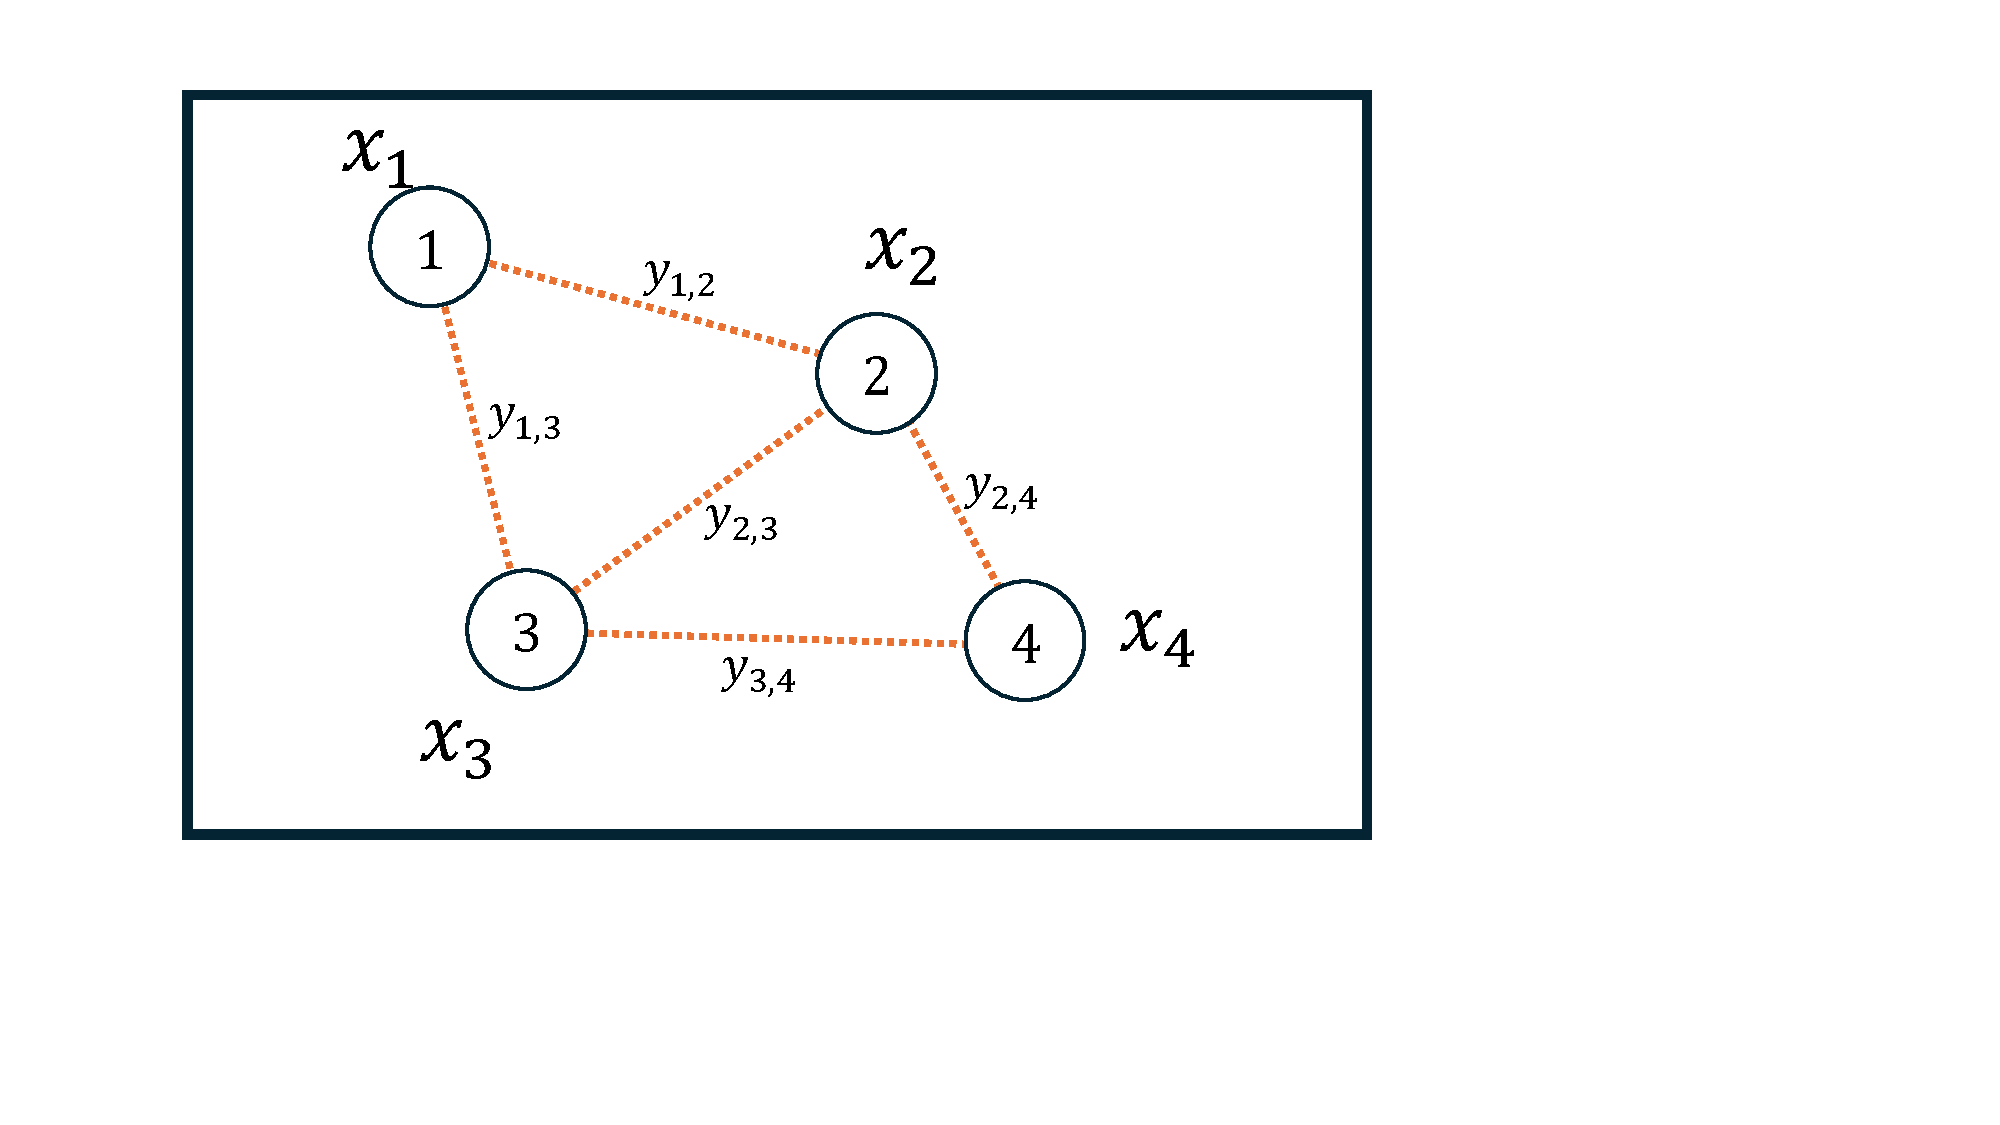
\includegraphics[width=\linewidth,trim=31mm 48mm 106mm 15mm, clip]{graph.pdf}
%     \caption{Problem reformulation. In the figure, we have a graph $\mathcal{G}=(\mathcal{V}, \mathcal{E})$ where the edges $(i, j) \in \mathcal{E}$ have weights $y_{i,j}$ and the vertices $k \in \mathcal{V}$ have positions $\bar{x}_k$.}
%     \label{fig:problem-graph}
% \end{figure}

In practice, it is rarely the case that the correspondences between robots are known without sophisticated identification algorithms using computer vision or other computationally complex methods. This is known as the anonymous localization problem, and it has been investigated by Franchi, Oriolo and Stegagno~\cite{anonymous_loc_1,anonymous_loc_2,anonymous_loc_3}. They developed a few algorithms to account for the missing correspondences by using statistical methods to simultaneously estimate multiple possible relative poses to determine the most likely correspondences. However, this markedly increases the complexity of the problem and will not be the focus of this project.

It will henceforth generally be assumed that while the measurements $y_{i,j}$ are not complete, i.e. all robots do not have measurements of every other robot, the correspondences are known. That is to say, for all measurements $y$, it is known which distance between two robots this is a measurement of. 

This problem is not new. One early approach to solve it was presented by Kruskal in \cite{Kruskal1964}. He proposed a measurement of good fit, or loss, named the stress function: 
\begin{align}
    \label{eq:kruskal-stress}
    S(\mathbf{x}^{(1)}, ..., \mathbf{x}^{(N)}) = \sum_{i,j} \left(
        \norm{\mathbf{x}^{(i)} - \mathbf{x}^{(j)}}_2 - y^{(i, j)}
    \right)^2
\end{align}
More accurately, Kruskal proposed a normalized version of equation~\ref{eq:kruskal-stress}, but for the purposes of this project the unnormalized version is sufficient. This function is non-convex, so iterative optimization algorithms such as gradient descent or ADMM generally converge to local minima, which necessitates a good initial guess. This algorithm will hereafter be called stress minimization in this paper.

In a companion paper, Kruskal provided a description of how to solve this problem using gradient descent~\cite{kruskal1964implementation}. Of interest to this project is the gradient that Kruskal determined. It should be noted that the stress function is non-differentiable and non-convex, so while Kruskal calls it a gradient, it is not necessarily so. Nonetheless, the stress minimization algorithm presented by Kruskal show empirically good results, so this this paper will continue with the slight abuse of notation. The gradient which will be used in the gradient descent variant algorithms implemented for this paper is derived from the one Kruskal presented in~\cite{kruskal1964implementation}. Given 
\begin{table}[ht]
    \centering
    \begin{tabularx}{\linewidth}{lX}
        $\mathbf{X} \in \R{2}$ & Current positions of robots \\
        $\hat{\mathbf{d}} \in \R{m}$ & Pairwise distance measurements between robots \\
        $\mathbf{d} \in \R{m}$ & Current distances between robots 
    \end{tabularx}
\end{table}
\FloatBarrier 
\noindent we get the gradient through
\begin{align}
    S^* &= \sum \left({d}_{i} - \hat{{d}}_{i}\right)^2 \\
    T^* &= \sum {d}_{i}^2 \\
    S   &= \sqrt{\frac{S^*}{T^*}} \\
    \mathbf{g}_k &= S \sum_{i} \frac{{d}_i - \hat{{d}_i}}{{d}_i} (\mathbf{X}_k - \mathbf{X}_{R(i)})
\end{align}
where $\mathbf{X}_k$ is row $k$ of $\mathbf{X}$, $\mathbf{g}_k$ is row $k$ of the gradient $\mathbf{g}$. Further, the sum is over all $i$ for which the measurement at row $i$ of $\hat{\mathbf{d}}$ is a measurement between robot $k$ and another robot $R(i)$.

In addition to how do calculate the gradient of the stress function, the paper also presents a way to determine the step sizes $\alpha_k$ in gradient descent:
\begin{align}
    \alpha_0 &\approx 0.2 \\
    S_k &= S(\mathbf{X}_k) = S(\mathbf{x}^{(1)}_k, ..., \mathbf{x}^{(N)}_k) \\
    \alpha_{k} &= \alpha_{k-1} \cdot \beta_k \cdot \gamma_k \cdot \delta_k \\
    \beta_k &= 4^{(\cos^3 \theta_k)} \\
    % \phi_k &= \frac{\left|\left|g_k\right|\right|_2\left|\left|g_{k-1}\right|\right|_2}{g_k^\top g_{k-1}} \\
    \theta_k &= (\text{Angle between last and current gradient}) \\
    \gamma_k &= \frac{1.3}{1 + (\min\{1, \frac{S_k}{S_{k-5}}\})^5} \\
    \delta_k &= \min\{1, \frac{S_k}{S_{k-1}}\}
\end{align}
This algorithm will from this point on be referred to as Kruskal's method or gradient descent with Kruskal step size. 

An alternative algorithm was proposed in~\cite{MDS_proposal} by De Leeuw. THe algorithm is called Scaling by MAjorizing a COmplicated Function (SMACOF), and it iteratively minimizes an upper bound of the stress function. Further investigated by De Leeuw in~\cite{SMACOF_convergence}, it has been proven to converge to a local minima of the stress function. However, this also requires a good initial guess to converge to a good optimum. 

% These methods, while prone to local minima, can still be useful due to their simplicity when given a sufficiently good initial guess. 

% In the field of sensor network localization, meaning many agents are deployed in an environment without knowledge of their positions, this problem has also been investigated. The main distinction with the robot localization problem is that authors generally assume that at least some positions known as anchors are known~\cite{WSN_collaborative,WSN_localization_techniques,optimization_WSN,WSN_stochastic}. 

% Authors in these fields present additional methods of solving this problem, with different advantages and drawbacks. One technique is Particle Swarm Optimization (PSO), where a collection of particles explore the n-dimensional space to find optima~\cite{WSN_particles}. Building on this, Zhou and Chen gave a stochastic approach in~\cite{WSN_stochastic}, which finds the global optimum with high probability. 

Recently, there has been some advancements in solving the distance-based localization problem. An algorithm developed by Halsted and Schwager dubbed the Riemannian Elevator has been proposed which has better guarantees than either stress minimization or SMACOF. This method relies on a tight modification of the stress minimization problem. The weighted stress minimization problem, where the distances have weights inversely proportional to their noise variance, given by 
\begin{align}
    \min_{\mathbf{X} \in \R{n \times d}} \sum_{i, j} \frac{w_{ij}}{2}\left(\norm{\mathbf{x}_i - \mathbf{x}_j} - \hat{d}_{ij}\right)^2
\end{align}
is modified by adding the unit vectors $y_{ij}$ and jointly optimizing
\begin{align}
    \min_{\substack{
        \mathbf{X} \in \R{n \times d} \\
        \mathbf{Y} \in (\mathcal{S}^{d-1})^m
    }} 
    \sum_{i, j} \frac{w_{ij}}{2}\norm{\mathbf{x}_i - \mathbf{x}_j - \hat{d}_{ij}\mathbf{y}_{ij}}^2
    \label{eq:re-prob3}
\end{align}
where $(\mathcal{S}^{d-1})^m$ the set of $m \times d$ matrices with unit vector rows, or equivalently, an oblique manifold. The following equivalent form of equation~\ref{eq:re-prob3} is the basis for the Riemannian elevator algorithm:
\begin{align}
    \min_{\mathbf{Y} \in (\mathcal{S}^{d-1})^m}
    \text{tr}(\mathbf{Q Y Y}^\top)
    \label{eq:re-prob4}
\end{align}
where 
\begin{align}
    \mathbf{Q} &= \hat{\mathbf{D}}^2 \mathbf{(W - WC(C^\top W C)^\dagger C^\top W)}
\end{align}
where $\mathbf{C}$ is the graph incidence matrix and where $\mathbf{W}$ and $\hat{\mathbf{D}}$ have $w_{ij}$ and $\hat{{d}}_{ij}$ respectively on their diagonals. This problem is relaxed by increasing the dimension of $\mathbf{Y}$ to $(\mathcal{S}^{m-1})^m$, then it is reparametrized into an SDP. By solving this SDP problem and then projecting the solution to $\mathbf{Y} \in (\mathcal{S}^{d-1})^m$, we get a good initial guess to the problem in equation~\ref{eq:re-prob4}, which can then be solved to a local minima with manifold optimization libraries~\cite{pymanopt}.